% -*- coding: utf-8 -*-
\chapter{Nucleophilicity Prediction with QTAIM and Conceptual DFT}

In this chapter, we investigate nucleophilicity prediction by combining
\gls{QTAIM} and Conceptual DFT. Our approach integrates these frameworks with
elements of statistical mechanics to offer a broader perspective on chemical
reactivity.

The computational tools developed here are closely related to those described
in the following chapter. This reflects our intention to provide a robust and
automated workflow that connects \gls{QTAIM} and \gls{CDFT} analyses in a
practical and reproducible way to analyse chemical reactivity. While
\gls{QTAIM} is fundamentally temperature-independent, Conceptual DFT,
particularly in its grand canonical formulation, allows us to consider
temperature effects explicitly ---although, of course, temperature remains a
macroscopic parameter, rather than an external perturbation applied directly to
a quantum system---. Both approaches ultimately rely on output from \gls{DFT}
calculations, where perturbatoins such as solvent effects can be incorporated.
These, in turn, influence the resulting \gls{QTAIM} and \gls{CDFT} properties.

To introduce further chemical realism, it is important to consider the presence
of multiple conformers in solution. Our workflow addresses this by sampling
geometries for each system as a function of temperature, thus capturing the
diversity of conformational behaviour encountered experimentally.

\newpage
To manage this complexity, we have developed a \python workflow that leverages
\plams for connectivity to \ams engines. As illustrated in
Figure~\ref{filter}, the workflow is initiated with plain text input files
defining the molecules of interest in SMILES format, along with calculation
parameters such as basis set, DFT functional, DFTB method, solvent,
temperature, and energy thresholds. All computed data are stored automatically
in a SQLite \database, facilitating systematic analysis and reproducibility. The
same infrastructure underpins our investigations of nucleophilicity, as well as
the entropy calculations described in Chapter~\ref{entropies}.

\vspace*{0.5cm}%
\begin{figure}[htbp]
    \centering
    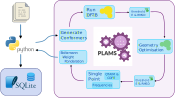
\includegraphics[width=0.9\textwidth]{diagramas/filter.pdf}
    \caption{Automated workflow developed for high-throughput calculations.
      The user provides input files containing the systems of interest and
      calculation parameters. All computed data are stored in a SQLite database
      for subsequent analysis.}
    \label{filter}
\end{figure}
\vspace*{0.5cm}%

The nucleophilicity project presented in this chapter is ongoing, and a journal
submission is in preparation. The latest version of the manuscript, prior to
submission, is included in the following pages.

\includepdf[pages=-]{paper.pdf}

